\documentclass{article}
\usepackage[utf8]{inputenc}
\usepackage[a4paper, total={6in, 8in}]{geometry}
\usepackage{setspace}
\onehalfspacing
\usepackage{graphicx}
\usepackage{hyperref}
\usepackage[english]{babel}
\usepackage{fancyhdr}



\pagestyle{fancy}
\fancyhf{}
\fancyhead[LE,RO]{Part 2: Digital Methods for Historians}
\fancyhead[RE,LO]{Theory Oriented Method}
\fancyfoot{}
\rfoot{Page \thepage \hspace{1pt} of 16}
\fancyfoot[LO,CE]{3.Semester BA}
\fancyfoot[CO,RE]{Andreas Viftrup Andersen}



\title{Voting Behaviours In the US 2020 Election}
\author{Andreas Viftrup Andersen}
\date{January 2021}

\begin{document}


\maketitle

\section{Abstract}
This paper serves as proof of concept of how R studio can be utilized to analyze a survey about voter frequency in the US 2020 election. It shows that voting frequency is related to income, level of education and race. It further shows that political orientation differentiates over set factors and it provides an insight in income level and degree of education of certain ethnic groups of the American population. The data analysis and plots were made by using R studio. It describes how the dataset was created and contains a critical evaluation of the methods used and results produced. 

\vspace{}
\textbf{Keywords:
Data analysis; Socioeconomic; Voting frequency }


\pagebreak

\tableofcontents

\pagebreak

\section{Introduction}
Data and statistics have become an integrated part of our daily lives. We are exposed to these when we must make a difficult decision, vote for a political party or understand complex problems and relations in the world. We use data science to grasp and understand the huge amount of information that are available and to make calculated and precise predictions about the future\footnote{Nate Silver Silver Nate, The signal and the noise : why most predictions fail, but some don't, ed. Nate Silver (New York, N.Y: Penguin Press, 2012). P. 5-7}.  We have also started to use data science in order to better understand the past. This project originates from my interest in American politics and socioeconomic topics. I have been interested in these topics since the 2008 presidential election of Obama. Over the years I have used the media FiveThirthyEight who uses data science in their news articles and predictions. In 2016 they and other election experts and polls failed to predict the election of Donald Trump. This came as a surprise for the majority of the established news media and political commentators as they were unable to predict how the American people would vote. That piqued my curiosity: How could they be so wrong? To understand a country and a culture is a difficult and complex task. Data science can be a useful tool in order to understand relations between socioeconomic factors and to understand behavior patterns of a population, but it requires a strong understanding of how to utilize data science correctly  in order produce valid and useful information, that can help us understand and better prepare for the future. 

\section{Problems and Background}
The voter turnout for the US 2020 presidential elections was at a historic high and is estimated to be between 66.4 and 72.1 percent of the eligible population.\footnote{"Voter turnout rate in the presidential election in the United States as of December 7, 2020," Statista, 2020, accessed 07-01, 2021, \url{https://www.statista.com/statistics/1184621/presidential-election-voter-turnout-rate-state/.}}  Yet a large percentage of the population abstain from voting in presidential or other elections. In any given US election, between 35 and 60 percent of the eligible voters don’t cast a ballot.\footnote{  "What is 'Voter Turnout'?," MIT Election Data Science Lab, accessed 07-01, 2021, \url{https://electionlab.mit.edu/research/voter-turnout.}}  The backbone of democracy is that eligible voters use their right to cast a ballot. Low turnout can cause a distortion in the election results as low turnout means low participation by certain groups of the population. Unequal participation means unequal representation and influences. This can create a self-reinforcing effect where certain citizens feels more and more that the system does not work for them and voting in elections is pointless.  The reasons for voter abstention are many and various and to examine who votes and who does not, is complex. It can be related to a wide variety of things such as; level of education, income, race and simple things like not being able to get off from work on election day. 
This study was conducted using R studio and first and foremost serves as a proof of concept of how data analysis of a survey can be conducted. It will provide insights in how a poll can be used to extract information of certain groups of respondents. This paper will also examine how various factors of the U.S. population such as education, race and income are related to voter turnout. Furthermore, it will provide insights in degree of education and income in relation to race and other factors. Since this paper uses a dataset that have been created and cleaned by professionals, this paper will only briefly touch the subject of data cleaning.\footnote{See Chapter 5: Data Acquisitions and Framework}    This project strives to make reproducible scripts and plots as this is a vital part of making data science.\footnote{  Julia S. Stewart Lowndes et al., "Our path to better science in less time using open data science tools," Nature Ecology & Evolution 1, no. 6 (2017/05/23 2017),
\url{https://doi.org/10.1038/s41559-017-0160.}}

\section{Software Framework}
This project was conducted on a Lenovo T530 Thinkpad with 8 GB RAM running Windows 10 OS. The data analysis and plots were created using R (4.0.3) and RStudio (3.167). Various software packages were installed in RStudio in order to complete the research. A full overview of installed software packages can be found in the GitHub repository assigned to this project. 

\section{Data Acquisition and Processing}
This project use data from a poll conducted between Sept. 15 to Sept 25 by Ipsos for the website FiveThirtyEight.\footnote{  "Data behind the story," FiveThirthyEight, 2020, accessed 07-01, 2021, \url{https://github.com/fivethirtyeight/data/tree/master/non-voters.}}   It was created using Ipsos Knowledge Panel.\footnote{  "Ipsos Knowledge Panel," Ipsos, 2021, accessed 07-01, 2021, \url{https://www.ipsos.com/en-us/solutions/public-affairs/knowledgepanel.}}  The poll examine various reasons for voting abstention. The poll was conducted among a sample of U.S. citizens that over sampled, young, Black and Hispanic respondents with 8.327 respondents. The poll was weighted according to general population benchmarks for U.S. citizens from the U.S. Census Bureau’s Current population survey, thus ending up with a sample size of 5.355 respondents. The respondents were then matched to a voter file for a more accurate understating of their voting history and placed in a voter category. Respondents who voted in all or all but one of the national elections they were eligible to vote in since 2000, were put in the ‘almost/always’ vote category. Those who voted in at least two elections, but fewer than all the elections they were eligible to vote in, were placed in the ‘sometimes’ category. Respondents who voted in no elections or just one, were put in the 'rarely or never' category.   Respondents who were only eligible to vote in three elections of fewer were dropped. The dataset used by this project is the final sample: 5.239 respondents who matched the voter file and whose voting history is verified. 
The dataset is thus in no need of further preparation or cleaning as respondents who did not match the requirements and whose voting history is unverified is dropped. However, the poll asks questions with multiple choice and giving respondents the possibility of not answering a question, thus ending up with missing values in certain questions. These values have been filtered out when working with this specific type of questions. See the script in the GitHub repository for further explanation.\footnote{"Final Project," GitHub, 2021, accessed 07-01, 2021, Line: 51-57} The poll is furthermore designed so respondents gets different questions depending on their previous answers. This leaves some respondents with missing values in certain questions and therefore in need of filtering. 

\section{Implementation and Empirical Results}
The purpose of this paper is to illustrate how polls and surveys can be used for data research.  As the dataset used by this paper is designed to be representative of the entire U.S. population, it can provide insights in a wide variety of things. The dataset contains information about the respondents that can be used to examine other topics not necessarily related to voter turnout. This chapter serves as a guide to the main script, which can be found in the linked GitHub repository. 

\subsection{Overview and Age Distributions of Respondents}
In order to examine the content of the survey, R can be utilized to quickly gain a broad overview of certain facets of the respondents. This can be used to examine if there is an overrepresentation of certain respondents; for example an overrepresentation of a certain race or highly educated respondents, thus making the dataset non-representative. Since the respondents in this dataset is not randomly selected, but designed to be representative of the U.S. population, it is not particularly relevant to examine if the dataset is representative, but in other cases this would be relevant. The script contains a couple of examples on how R can provide insights in respondents.\footnote{"Final Project." Line:14-38}  An example of how R can be utilized to provide insights in the respondents is to examine the age distribution of respondents. The code used to generate the plot below can be found in the GitHub repository.\footnote{"Final Project." Line: 30-38}      
\begin{figure}[!ht]
  \centering
  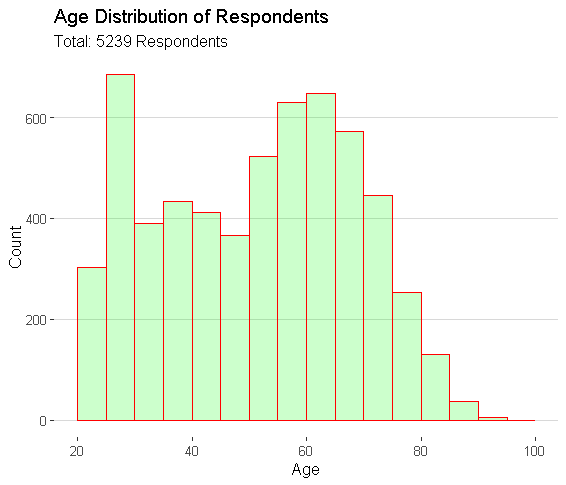
\includegraphics[width=\textwidth]{age_distribution.png}
  \caption{Age Distribution}
\end{figure}
\pagebreak


\subsection{Voting Frequency}
Since the dataset contains valid and confirmed information about the voting history of respondents, R can be utilized in different ways to provide an insight in voting frequency. By doing this one can examine how often respondents vote relative to their income group, level of education or race. The dataset was originally created to examine why many Americans don’t vote in national elections and by utilizing R this way, one can get a broad overview of voting frequency relative to different factors. Figure 2 below is an example of voting frequency relative to age.\footnote{"Final Project.". Line: 99-113}  

\begin{figure}[!ht]
  \centering
  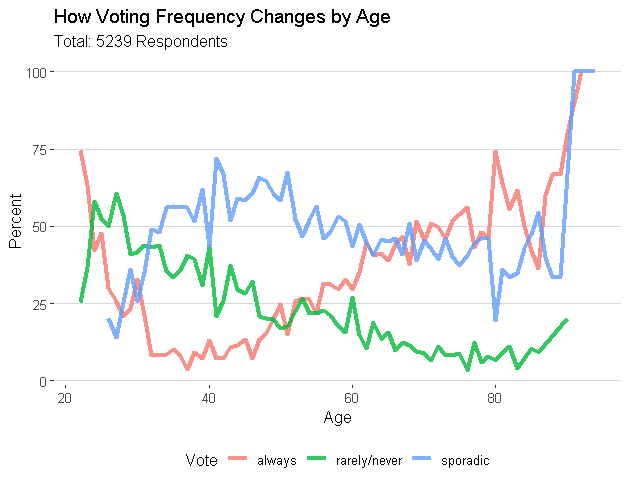
\includegraphics[width=\textwidth]{vote_age.png}
  \caption{Voting Frequency relative to age}
\end{figure}
\pagebreak

The plot in figure 2 is not particularly useful, since voting frequency above age 80 is misleading or hard to interpret. This is because the sample size of respondents above 80 is relatively low compared to other age groups, thus making the plot inaccurate or misleading when examining voting frequency relative to age, or at least unable to produce valid information. This is an example of how one needs to be attentive and critical when plotting data, as a to small sample size can lead to inaccurate or misleading data. A better way is to examine voting frequency is relative to income, or other factors where the sample size is sufficient. In the script are examples of how one can examine voter frequency relative to race, education and income.\footnote{"Final Project." Line:94-167} As can be seen from figure 3 below voting frequency changes significantly over income groups. Respondents with income above \$125k or more votes more often that respondents who earns less than \$40k.\footnote{"Final Project.". Line: 133-149} 

\begin{figure}[!ht]
  \centering
  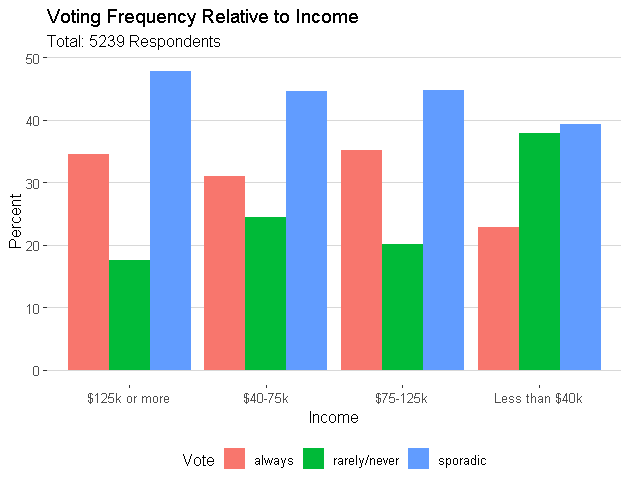
\includegraphics[width=\textwidth]{vote_income.png}
  \caption{Voting Frequency and Income}
\end{figure}
\pagebreak

\subsection{Other Useful Ways of Utilizing R}
The respondents in the survey answered several questions about their political orientation, income, degree of education etc. This information can be used to examine other socioeconomic topics that are not necessarily related to voting frequency.  Figure 4 below is an example of an examination of political orientation related to race. It shows that Joe Biden enjoys the support of mostly all non-whites and white voters are more divided but leaning towards Donald Trump.

\begin{figure}[!ht]
  \centering
  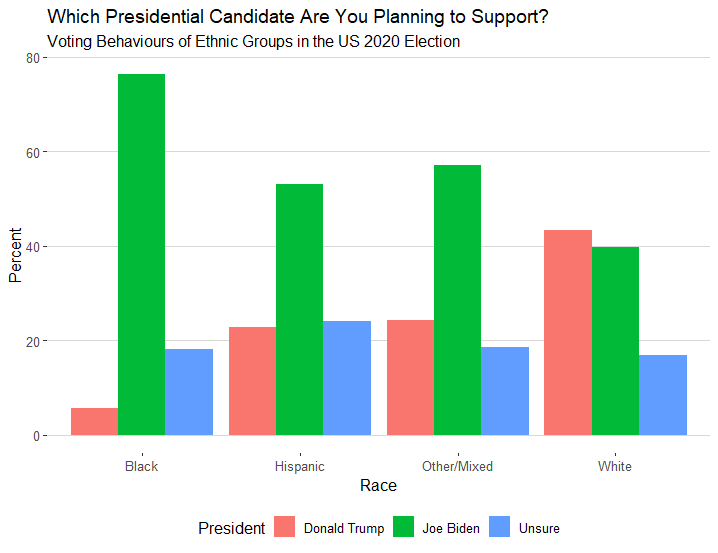
\includegraphics[width=0.9\textwidth]{race_president.png}
  \caption{Ethnic Groups and Presidential Candidate}
\end{figure}
\pagebreak

The script shows examples of how these socioeconomic topics can be examined using R.\footnote{"Final Project.". Line: 76-92}  The GitHub repository contains a folder where all the plots created can be found.
Working with this dataset in R proved to be more complicated than first anticipated. To fully understand how respondents answered questions I had to access the codebook provide by Ipsos, that made me able to interpret and understand the answers of the questions. The answers in the dataset is listed as numbers instead of text. I therefore had to use the function in R called ´levels´ which allowed me to change the set numbers to the corresponding answers with text.\footnote{"Final Project.". Line:61-63}  E.g. when working with presidential candidates, Donald Trump corresponded with the number 1, Joe Biden with 2 and unsure with 3. By using the levels function I was able to rename these numbers into their corresponding presidential candidate thus making the data easier to understand when plotting. Another useful function is the ´mutate´ function that allowed me to create a new variable from my dataset. This function was used throughout the entire script when I wanted to examine how multiple variables where related to each other or group data for a clearer insight

\section{Critical Evaluation}
This project use data from a survey conducted by Ipsos for the website FiveThirthyEight. Ipsos is a multinational market research and consulting firm that was founded in 1975. The survey was created by using Ipsos KnowledgePanel, a probability-based online panel that is recruited to be representative of the U.S. population.\footnote{  Wolfe, "Data behind the story."}  According to their own website: \textbf{\textit{“The KnowledgePanel provides a statistically valid representation of the U.S. population as well as many under-researched and often harder-to-reach populations.”}}\footnote{  "Ipsos Knowledge Panel."}  The KnowledgePanel consist of 60.000 members with over 2 thousand profile variables. The participants of the panel are invited by mail after being selected through a single sampling file of the United States Postal Service, that covers almost all the U.S. It is not possible to volunteer. Ipsos has many years of experience in data science and in conducting online research programs and boast of ensuring accuracy with an industry leading representative random sample, exceptional response rates and coverage. FiveThirthyEight is a news media that focuses on opinion poll analysis, politics and economics blogging. The website publishes articles that typically focuses on creating or analyzing statistical information.\footnote{  "FiveThirthyEight," ABC New Internet Ventures, accessed 07-01, 2021, \url{https://fivethirtyeight.com/.}}  The dataset used by this project features in an article on FiveThirtyEight called ‘Why Many American Don’t Vote’.\footnote{  "Why Many Americans Don't Vote," ABC News Internet Ventures, 2020, accessed 07-01, 2021, \url{https://projects.fivethirtyeight.com/non-voters-poll-2020-election/.}}   Since the dataset have been created and prepared to use by experts with many years of experience, the quality of the dataset must be regarded as high. Ipsos and the KnowledgePanel focus explicitly on creating data that are representative of the population of the U.S and can be used by a wide variety of clients. This strengthens the representativeness and reliability of the dataset. Furthermore, the data have been used to produce articles by the highly regarded website FiveThirthyEight. The purpose of this paper was to illustrate how R can be used to extract information from a poll or survey and to examine voting frequency in relation to a variety of socioeconomic factors in the American population. A lot of time was spent learning how to use R functions to examine the relations I wanted. The information I extracted from the plots are by no means groundbreaking or particularly revealing and mostly confirms already existing conclusions. In order to get more in-depth knowledge of voting frequency and why many Americans don´t vote a larger knowledge than I currently possess is required. Still I managed to extract some information that provides a very broad overview of socioeconomic relations in the American population. The process of learning R have overall been entertaining, but also very challenging. I often ran into problems I could not solve myself at first, but by searching online and consulting my colleagues and course instructors I managed to move forward. I especially found the YouTube channel ´Dataslice´ helpful.\footnote{  "Data tutorials, tips & tricks," Dataslice, accessed 07-01, 2021, \url{https://www.youtube.com/channel/UCBV194XNr6CIQCCuw1v2rMQ.<}}  I had some experience with programming before I started on this course. From that I learned that the trail-and-error method brings you a long way. 

\section{Conclusion}

The purpose of this paper was to illustrate how data analysis of a survey can be conducted and to provide insight in certain socioeconomic factors in relation to voting frequency. Furthermore, it was to provide insight in degree of education and income in relation to race and other factors. The dataset was created by professionals and therefore in no need of further cleaning and preparation. From the analysis it shows that voting frequency differentiates over several variables such as race, income and level of education. Highly educated and high-income respondents vote more often than respondents, that are less educated or have low income. It can not be concluded that voting frequency is directly related to these factors, but a pattern can be detected. Further examination is needed to fully understand these relations. The analysis provides an insight in socioeconomic relations such as income and race.  
To execute this analysis, I had to learn and utilize a wide variety of functions in R. Learning how to use the mutate and levels function was critical in order to get the desired results. This allowed me to create new variables from the dataset and to select, filter, group and arrange data. The mutate function is a part of the dplyr package, which is an add-on to R that include a wide variety of useful functions. This project further taught me how to efficiently search for information online on certain problems and were to look for help. The trail-and-error approach and mindset also proved helpful.
\pagebreak
\section{References}
\begin{itemize}

    \item "Why Many Americans Don't Vote." ABC News Internet Ventures, 2020, accessed 07-01, 2021, \url{https://projects.fivethirtyeight.com/non-voters-poll-2020-election/}
    \item "Final Project." GitHub, 2021, accessed 07-01, 2021, \url{https://github.com/Digital-Methods-HASS/au539080_Andreas_Viftrup/blob/main/Final%20Project/final_project.R}
        \item "Data Tutorials, Tips & Tricks." Dataslice, accessed 07-01, 2021, \url{https://www.youtube.com/channel/UCBV194XNr6CIQCCuw1v2rMQ}
    \item "Voter Turnout Rate in the Presidential Election in the United States as of December 7, 2020." Statista, 2020, accessed 07-01, 2021, \url{https://www.statista.com/statistics/1184621/presidential-election-voter-turnout-rate-state/}
    \item "Fivethirthyeight." ABC New Internet Ventures, accessed 07-01, 2021, 
    \url{ https://fivethirtyeight.com/}
    \item "Ipsos Knowledge Panel." Ipsos, 2021, accessed 07-01, 2021, \url{https://www.ipsos.com/en-us/solutions/public-affairs/knowledgepanel}
    \item Lowndes, Julia S. Stewart, Benjamin D. Best, Courtney Scarborough, Jamie C. Afflerbach, Melanie R. Frazier, Casey C. O’Hara, Ning Jiang, and Benjamin S. Halpern. "Our Path to Better Science in Less Time Using Open Data Science Tools." Nature Ecology & Evolution 1, no. 6 (2017/05/23 2017): 0160. \url{https://doi.org/10.1038/s41559-017-0160. https://doi.org/10.1038/s41559-017-0160}
    \item Nate, Silver. The Signal and the Noise : Why Most Predictions Fail, but Some Don't. Edited by Nate Silver. New York, N.Y: Penguin Press, 2012.
    \item "What Is 'Voter Turnout'?" MIT Election Data Science Lab, accessed 07-01, 2021, \url{https://electionlab.mit.edu/research/voter-turnout}
    \item "Data Behind the Story." FiveThirthyEight, 2020, accessed 07-01, 2021, \url{https://github.com/fivethirtyeight/data/tree/master/non-voters}
    
\end{itemize}
\pagebreak

\section{Required Metadata}

\begin{table}[ht]
\setlength{\tabcolsep}{20pt}
\renewcommand{\arraystretch}{1.5}
    \centering
    \begin{tabular}{p{0.10\linewidth} | p{0.40\linewidth} | p{0.40\linewidth}}
    \textbf{Nr.}     & \textbf{Software Metadata Description}       & \textbf{Information}  \\ \hline
    S1 & Current software version & R (4.0.3) and RStudio (3.167) \\
    S2 & Permanent link to executables of this version & \url{https://github.com/Digital-Methods-HASS/au539080_Andreas_Viftrup/blob/main/Final%20Project/final_project.R} \\
    S3 & Legal Software License & CC-BY-SA\\
    S4 & Computing platform/Operating system & Windows 10 OS \\
    S5 & Installation requirements and dependencies for software not used in class & None \\
    S6 & Support email for questions & andreasviftrup@gmail.com
    \end{tabular}
    \caption{Software Metadata }
    \label{tab:my_label}
\end{table}

\begin{table}[ht]
\setlength{\tabcolsep}{20pt}
\renewcommand{\arraystretch}{1.5}
    \centering
    \begin{tabular}{p{0.10\linewidth} | p{0.40\linewidth} | p{0.40\linewidth}}
    \textbf{Nr.}     & \textbf{Software Metadata Description}       & \textbf{Information}  \\ \hline
    D1 & Link to codebook & \url{https://github.com/Digital-Methods-HASS/au539080_Andreas_Viftrup/blob/main/Final%20Project/nonvoters_codebook.pdf}  
      \end{tabular}
    \caption{Data Metadata }
    \label{tab:my_label}
\end{table}
\pagebreak

\section{Learning Journal}

\subsection{Week 44}
\subsubsection{Thoughts / Intentions}

I am currently reading the literature, but I don't understand very much. I have no idea what regular expressions is. The literature on data organizations makes better sense for me though. I like data science and find it pretty interesting.  I have some experience with it, but I've never worked with regular expressions so this is new. I´ve mostly worked in Python and MatLab. 

\subsubsection{Action}

\begin{itemize}
\item Downloaded all the required software for the course. It seems to works fine, but I will probably consult the instructors just to be sure.  
\item Read Introduction for Data Organization in Spreadsheets for Social Scientists
\item Started making the exercises alone, but eventually had to consult my colleagues. I made some progress and after the lecture I have a better understanding of what it does. 
\item The hands-on session was useful. I really need to pay attention, because this seems hard.
\end{itemize}

\pagebreak{}

\subsection{Week 46}
\subsubsection{Thoughts / Intentions}
I am struggling with this course. I like the theoretical approach of the lectures on how data science can be relevant for historians and would very much like to be able to use digital tools. But learning and using the programs we are introduced to, takes a lot of time and is very frustrating. 

I don't really see the purpose of Git/Bash for this course. It seems irrelevant, at least for the type of project I am currently thinking about doing. I've been looking online for datasets that could be of interest. I´ve found a  subreddit where people upload datasets for various sources. Some of thees looks very interesting. I should look more into that. 

\subsubsection{Action}

\begin{itemize}
\item Looking into datasets for my final project.  
\item Did the introduction to Git. What is that? I'm struggling to make sense of this.
\item Tried to read the course literature by Neal Stephenson, but I did not finish.
\item Did the homework for week 46. Took a very long time, but I managed to finish all the tasks. Had to consult instructors and colleagues numerous times. I still don't understand what the purpose of this software is, but I managed to solve the exercises.   
\end{itemize}

\pagebreak{}

\subsection{Week 47}
\subsubsection{Thoughts / Intentions}
Started with R studio. It reminds me of Python and MatLab, which I have some experience working with. This makes the progress less frustrating. Happy to be done with Git/Bash and moving on to something more familiar. 

Started doing the exercises. Manage to get a long way myself after reading the tutorials carefully.
Created my GitHub account. I have no experience with GitHub, but heard of it before. Will have to spent some time learning how to use and navigate it. Manage to upload my screenshot of R for the homework exercise.

\subsubsection{Action}

\begin{itemize}
\item Continued to look into datasets for my final project. I am interested in US politics and voting behaviour. Been reading on the website FiveThirthyEight, that makes a lot of news articles based on data. Maybe I could do something like that? 
\item Finished the exercises with minor problems. Felt good to be able to work with R after reading the tutorial.
\item Sat up my GitHub account. 
\item Forgot to do the peer review on Blackboard.  
\end{itemize}



\end{document}



